Here first the limitations of Scikit-learn predefined ML models - Logistic Regression(LR) and Multi-Layer-Perceptron(MLP), are described. The Logistic Regression Model seems to work almost perfectly with all 3 classes when the bad region size is $5\times5$ (as in \autoref{Occupancymaps5x5}) with either the same or randomized location. When the bad region size is 1x1 like in \autoref{Ocuppancymaps1x1} the LR Model performs poorly with an accuracy of approximately 20\%.
 The MLP does not seem to work in any of the used cases that are studied as it always performs poorly with an accuracy of $\approx 40\%$.

\begin{figure}[h]
\centering
\begin{subfigure}[t]{.316\textwidth}
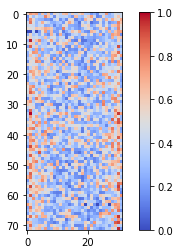
\includegraphics[width=\textwidth]{Good_image_1x1.png}
\caption{}
\end{subfigure}
\begin{subfigure}[t]{.305\textwidth}
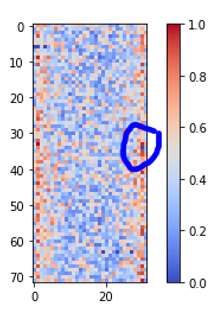
\includegraphics[width=\textwidth]{Dead_image_1x1.png}
\caption{}
\end{subfigure}
\begin{subfigure}[t]{.3\textwidth}
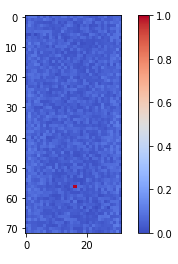
\includegraphics[width=\textwidth]{Hot_image_1x1.png}
\caption{}
\end{subfigure}
\vspace{5mm}
\caption{Occupancy Maps with 1x1 bad regions. A) Good image B) Dead image C) Hot image\label{Ocuppancymaps1x1}}
\end{figure}

Also, the use of Scikit-learn’s library is limited in comparison with the Keras module since one cannot customize the structure of the ML model with detail. Moreover, Keras is an ML library designed for developing deep neural networks. Hence it was decided to use Keras primarily for the creation of the model.
 With the Keras library, numerous models were designed with both, SL method and SSL learning method. Using SL method, we are interested in detecting anomalies and classifying what type of anomaly is seen. With SSL method, we are interested in looking at the error of the reconstruction of an image to give an idea that the image given can be considered good or that it might have some unseen anomalies

\section{SL Models for known anomalies in the HCAL data for DQM}
We considered three SL Models for classification of known anomalies in the HCAL data for DQM. 
These models are based on Convolutional Neural Networks and differ in the number of layers utilized, their ordering and number of units in each layer. The Models and the corresponding results are described below.


\subsection{Two Convolutional Layers for binary classification}
Several variations of the two Convolutional Layers Model were tested and optimized on the DQM data. This led to an optimal value of 8 units/neurons in the Convolutional layers. 
The detail of selecting the number of units per layer is of great importance to find a balance between efficiency and complexity of a model. More complex models (more layers and connections) are “heavy” to train in terms of computational cost, provide better results and are prone to “overfitting” to the training data.
 Simpler models (fewer layers and connections) are quicker to train, efficient and computationally economic. However, simpler models are more likely to “underfit” to the data. The \autoref{fig:2convlayermodel} below shows a code snippet with this model.
\autoref{fig:2convlayermodelfixedresults} below shows the learning curve for this model trained with Good and Hot images for fixed $5\times 5$ location and the corresponding Confusion Matrix.

\autoref{fig:2convlayermodelrandomresults} shows the learning curve for this model trained with Good and Hot images for fixed $5\times5$  location and the corresponding Confusion Matrix.

\begin{figure}
\begin{center}
    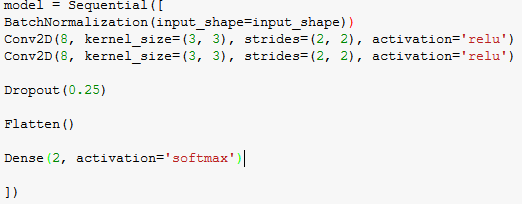
\includegraphics[width=.9\textwidth]{2_conv_layers_model.png}
\end{center}
\caption{Two Convolutional Layers Model\label{fig:2convlayermodel}}
\end{figure}


\begin{figure}
\centering
	\begin{subfigure}{.45\textwidth}
 	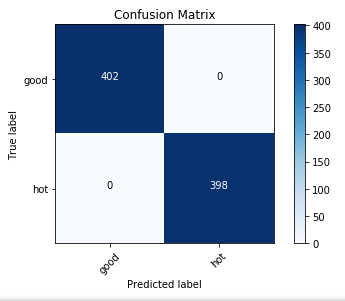
\includegraphics[width=\textwidth]{CM_2x2_with_5x5_good_hot_fixed.png}
	\end{subfigure}
	\begin{subfigure}{.45\textwidth}
	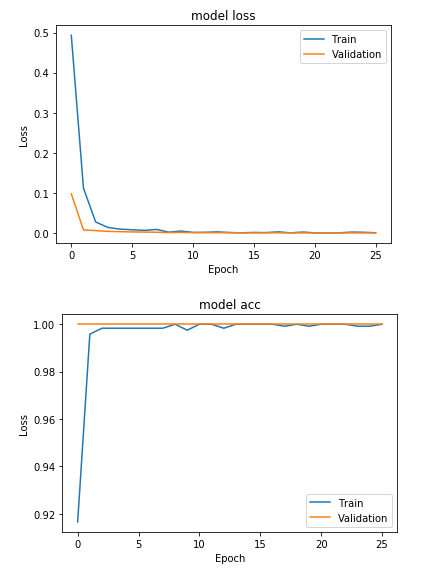
\includegraphics[width=\textwidth]{Learning_curve_5x5_good_hot_fixed.png}
	\end{subfigure}
	\caption{Confusion Matrix results and Learning curve
	 for $5\times 5$ damaged area with on the same location for all trials\label{fig:2convlayermodelfixedresults}}
 \end{figure}
 
 \begin{figure}
 	\begin{subfigure}{.45\textwidth}
 		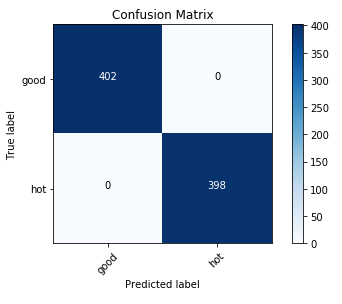
\includegraphics[width=\textwidth]{2x2CMwith_5x5_good_hot_random.png}
 	\end{subfigure}
 	\begin{subfigure}{.45\textwidth}
 	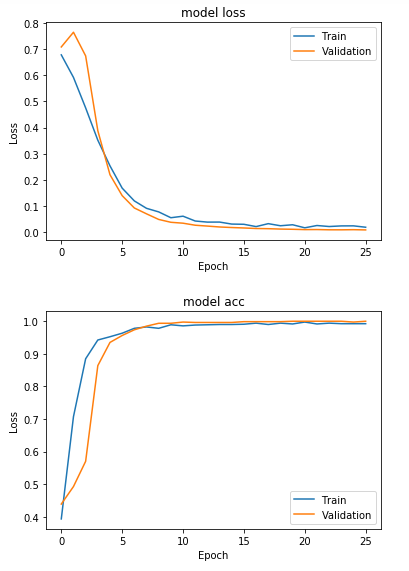
\includegraphics[width=\textwidth]{Learning_curve_5x5_good_hot_random.png}
 	\end{subfigure}
 \caption{Confusion Matrix results and Learning curve
	 for $5\times5$ damaged area with on the random location for all trials\label{fig:2convlayermodelrandomresults}}
 \end{figure}
 

\begin{figure}
	\begin{subfigure}{.5\textwidth}
 		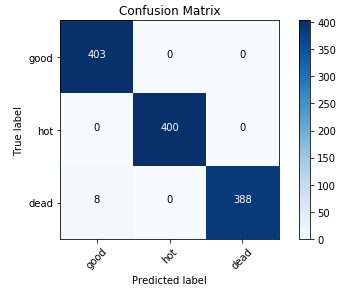
\includegraphics[width=\textwidth]{3x3CMwith_5x5_good_hot_dead_random.png}
 	\end{subfigure}
 	\begin{subfigure}{.45\textwidth}
 	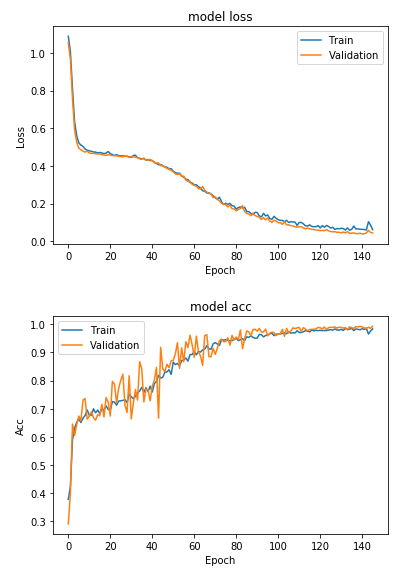
\includegraphics[width=\textwidth]{Learning_curve_5x5_good_hot_dead_random.png}
 	\end{subfigure}
 \caption{Confusion Matrix results and Learning curve
	 for $5\times5$ damaged area with an extra class to identify with random location for all trials\label{fig:2convlayermodelGHDrandomresults}}
 \end{figure}
 
\autoref{fig:2convlayermodelGHDrandomresults} shows the learning curve for this model trained with Good, Hot and Dead images for random $5\times5$ location and the corresponding Confusion Matrix

\autoref{fig:2convlayermodelGHD1x1randomresults} shows the learning curve for this model trained with Good, Hot and Dead images 
for random 1x1 location and the corresponding Confusion Matrix. 
The corresponding learning curves and confusion matrix for a fixed location for 3-class 
(Good, Hot, Dead) configuration give the same behavior as 2-labels (Good, Hot) images



\begin{figure}
\begin{subfigure}{.5\textwidth}
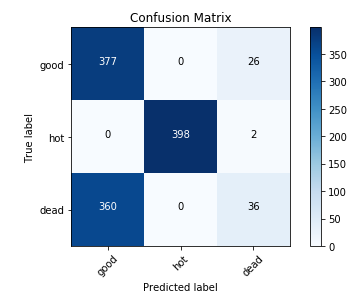
\includegraphics[width=\textwidth]{3x3CMwith_1x1_good_hot_dead_random.png}
\end{subfigure}
\begin{subfigure}{.45\textwidth}
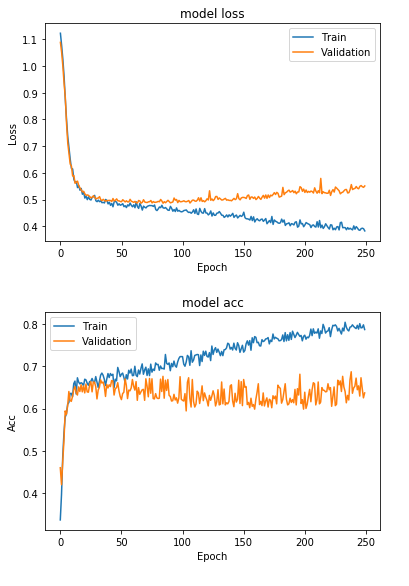
\includegraphics[width=\textwidth]{Learning_curve_1x1_good_hot_dead_random.png}
\end{subfigure}
\caption{Confusion Matrix results and Learning curve for $1\times1$ damaged area with random location for all trials
 \label{fig:2convlayermodelGHD1x1randomresults}}
\end{figure}
	
	
In a more realistic scenario, the problems with HCAL DQM would be more granular i.e. $1\times1$ type. 
When this model is tested for problematic channels in $1\times1$ configuration the learning curves for the training (blue) and validation (orange) sets depart after few epochs as shown in Figure 12 (right part).
From the left part of the figure, dividing the sum of numbers along the diagonal (377+398+36) by the sum of all the numbers in the matrix gives ~1/3. This demonstrates that the model is “overfitting” to the training set and misclassifies images $\approx 33\% $ of times. Hence, we consider adding a Convolutional layer to gain more prediction accuracy as shown in the next section.	
	
	
	
	
In this section the results for the final estimation of the of the Z$\rightarrow\nu\bar{\nu}$ are presented. The current study includes preliminary results using only data obtained at the CMS detector during 2016. The results for this study are intended to confirm the assumption that the additional $\gamma+$jets control region introduced in this analysis reduce the overall uncertainties obtained in the 2016 analyses (described in \autoref{AnalysisChap}). Furthermore, this study is intended as a benchmark for future analyses of the SUSY stop group based in Fermilab and will be the method used for the 2017 CMS data.

\subsection{Systematics}\label{systematics}

Two categories of uncertainties for the Z$\rightarrow\nu\bar{\nu}$ prediction are considered: uncertainties that are associated to the use of MC simulation and the uncertainties specifically associated to the background prediction method. Several sources are acknowledged in the first category mentioned such as PDF and renormalization/factorization scale choices, jet and $p_\text{T}^{miss}$ energy scale uncertainties b-tag scale factor uncertainties, and trigger efficiency uncertainties. Given that the simulation sample is normalized to data in the tight control region, uncertainties associated with the luminosity and cross-section are excluded. In addition, the overall Z$\rightarrow\nu\bar{\nu}$ statistical uncertainty from MC simulation is also taken into account.\\

\begin{figure}[H]
\begin{center}
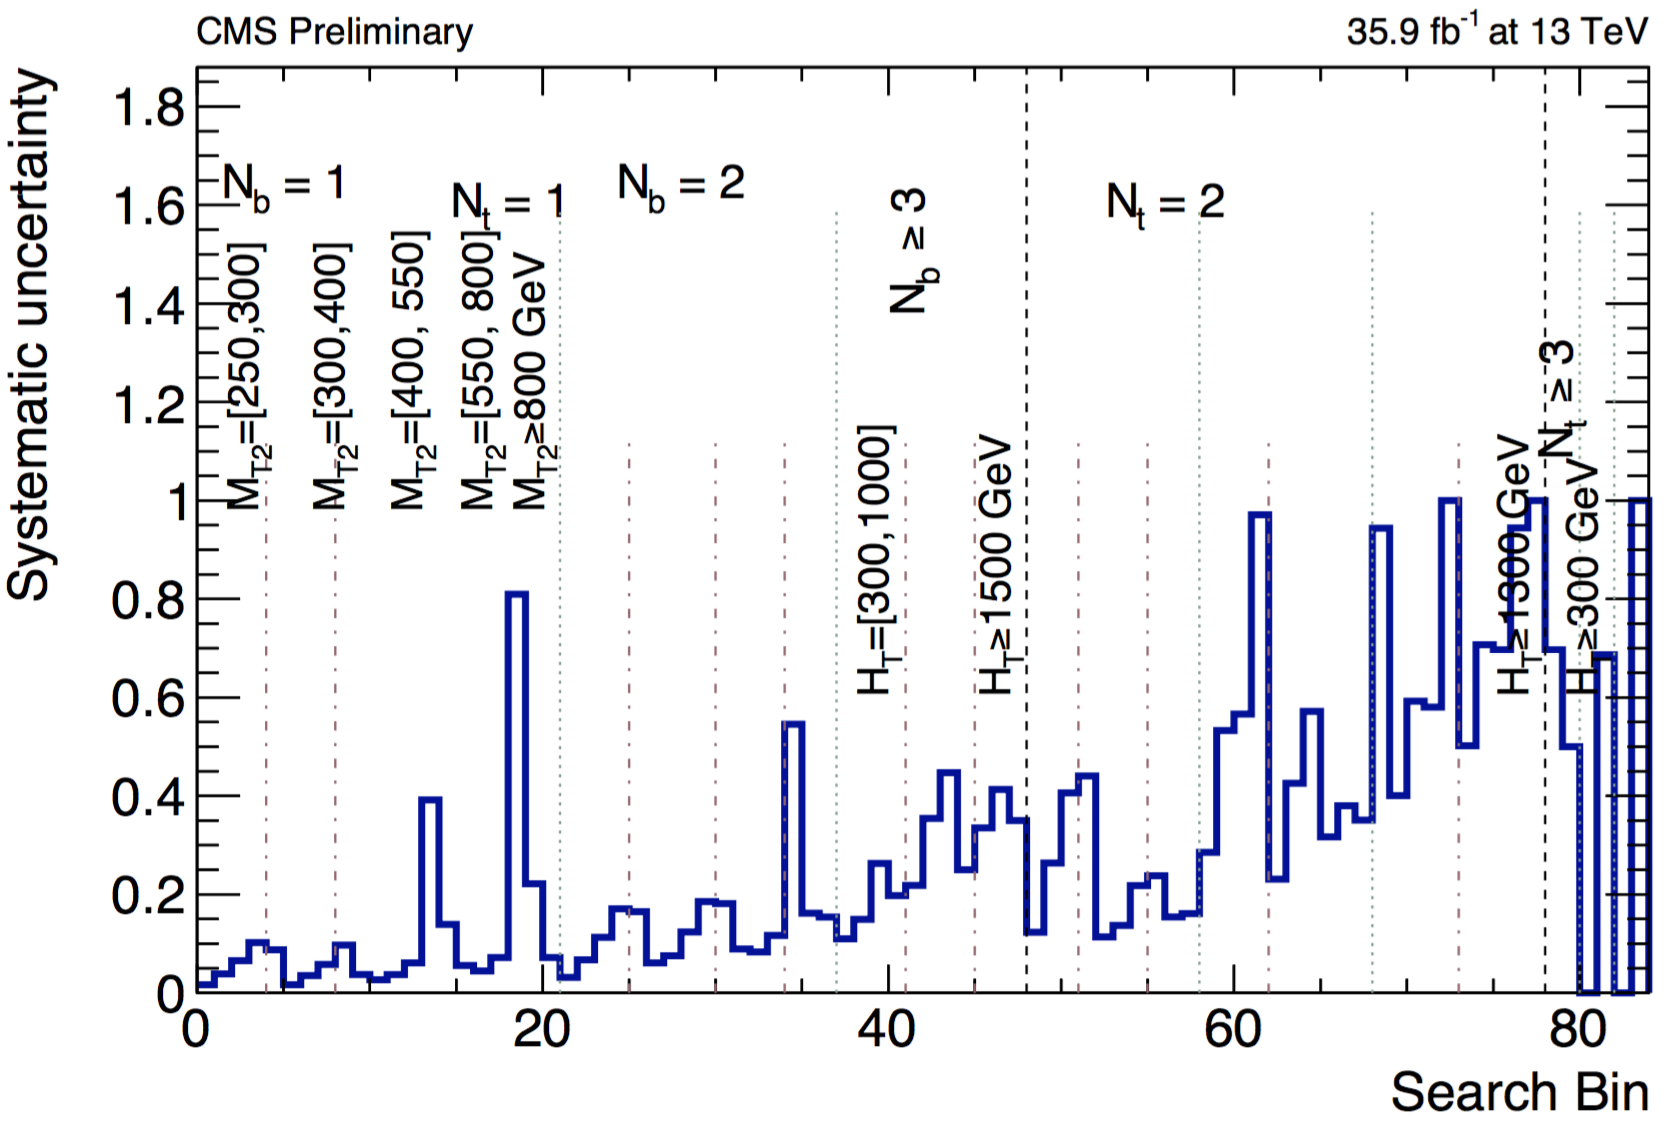
\includegraphics[width=0.8\textwidth]{UncZnunu}
\end{center}
\vspace{-1em}
\caption{Systematic uncertainty in the final prediction, as a function of the search bin, associated to the MC statistics.}
\label{UncZnunu}
\end{figure}

The statistical uncertainty associated with each bin in the MC is propagated as a systematic uncertainty. The relative uncertainty per bin can be see in \autoref{UncZnunu}. It shows that the uncertainties for the MC vary from as low as 1\% up to 81\% and even 100\% in some regions. Since the final estimation is scaled using the global normalization factor from the tight $\mu\mu$ control region ($R_{norm}$), the total uncertainty, due to limited amounts of events in data, is propagated in the final prediction. This is also true for the $S_\gamma$($N_j$) scale factor, in which the residual differences in search variables other than $N_j$ are evaluated in the loose photon control region. Both the uncertainty arising from the $N_j$ re-weighting as well as the residual differences are evaluated together. The uncertainty from $R_{norm}$ is propagated as a flat value of 7.9\% uncertainty per each search bin.

\subsection{Z$\rightarrow\nu\bar{\nu}$ Estimation for the Search Bins}

The final estimation for the Z$\rightarrow\nu\bar{\nu}$ background calculated for all 84 search bins is shown in \autoref{results}. The statistical uncertainty in bins that have zero events is treated as the average weight (the sum of the weights squared over the weight) times the poisson error on 0 which is 1.8. This average weight is calculated on the basis of a relaxed cut in which $N_b \geq 2$ is required. For comparison, a cut in which $N_t > 2$ where two tops are fake for the Z$\rightarrow\nu\bar{\nu}$ is used.

\begin{figure}[H]
\begin{center}
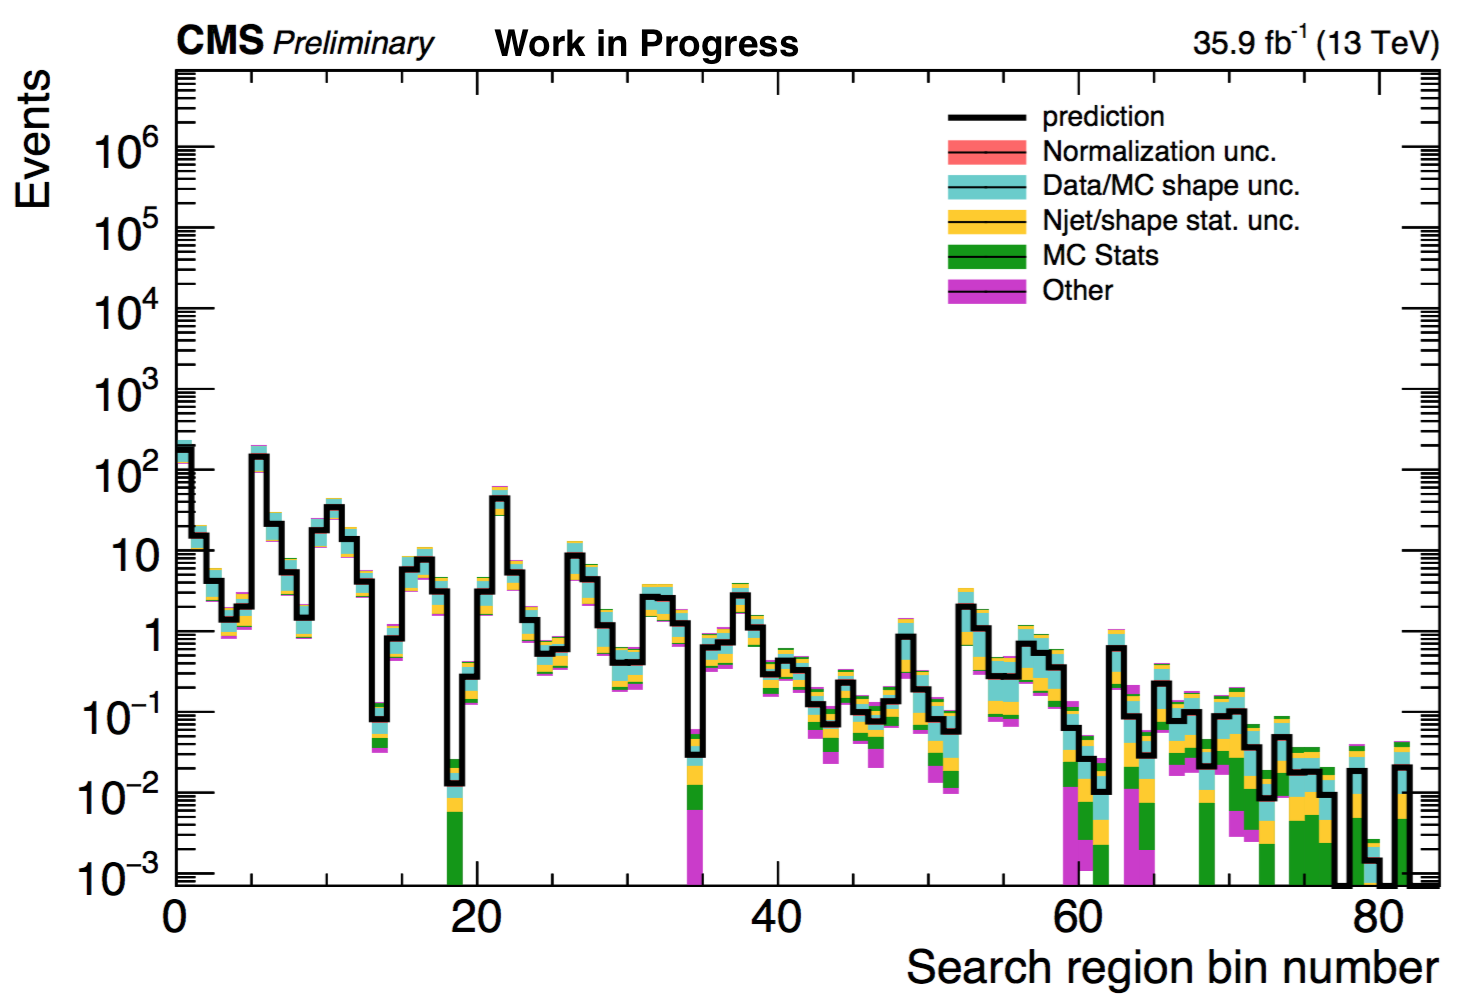
\includegraphics[width=0.8\textwidth]{Results.png}
\end{center}
\vspace{-1em}
\caption{Z$\rightarrow\nu\bar{\nu}$ background prediction for all search bins, including the breakdown of the various uncertainties.}
\label{results}
\end{figure}

